\ChapterImagePrelim[cap:cronograma]{Cronograma}{./images/fondo.png}\label{cap:cronograma}
\mbox{}\\
\noindent
En la figura~\ref{fig:cronograma} se expone el cronograma de actividades del proyecto, el cual constituye una herramienta de planificación que organiza las fases metodológicas a lo largo de seis meses de ejecución. El recurso muestra cómo, desde las primeras semanas, se inicia el proceso con la fase de reconocimiento de necesidades, la cual sienta las bases para las etapas posteriores. A continuación, se desarrollan la identificación y caracterización de las tecnologías de \VBC, seguidas de la comprobación de sus características y del análisis mediante la técnica \DAR, lo que permite garantizar una selección fundamentada. Posteriormente, se contempla el diseño de la especificación arquitectónica, que antecede a la implementación de un prototipo funcional y a la validación del producto mínimo viable \PMV. Además, el cronograma resalta la construcción del informe final como una actividad transversal que acompaña todo el proceso. De este modo, la figura no solo facilita la visualización de la secuencia y duración de las fases, sino que también evidencia la interdependencia y la progresión lógica de las tareas necesarias para alcanzar los objetivos del proyecto.
\begin{figure}[H]
    \centering
    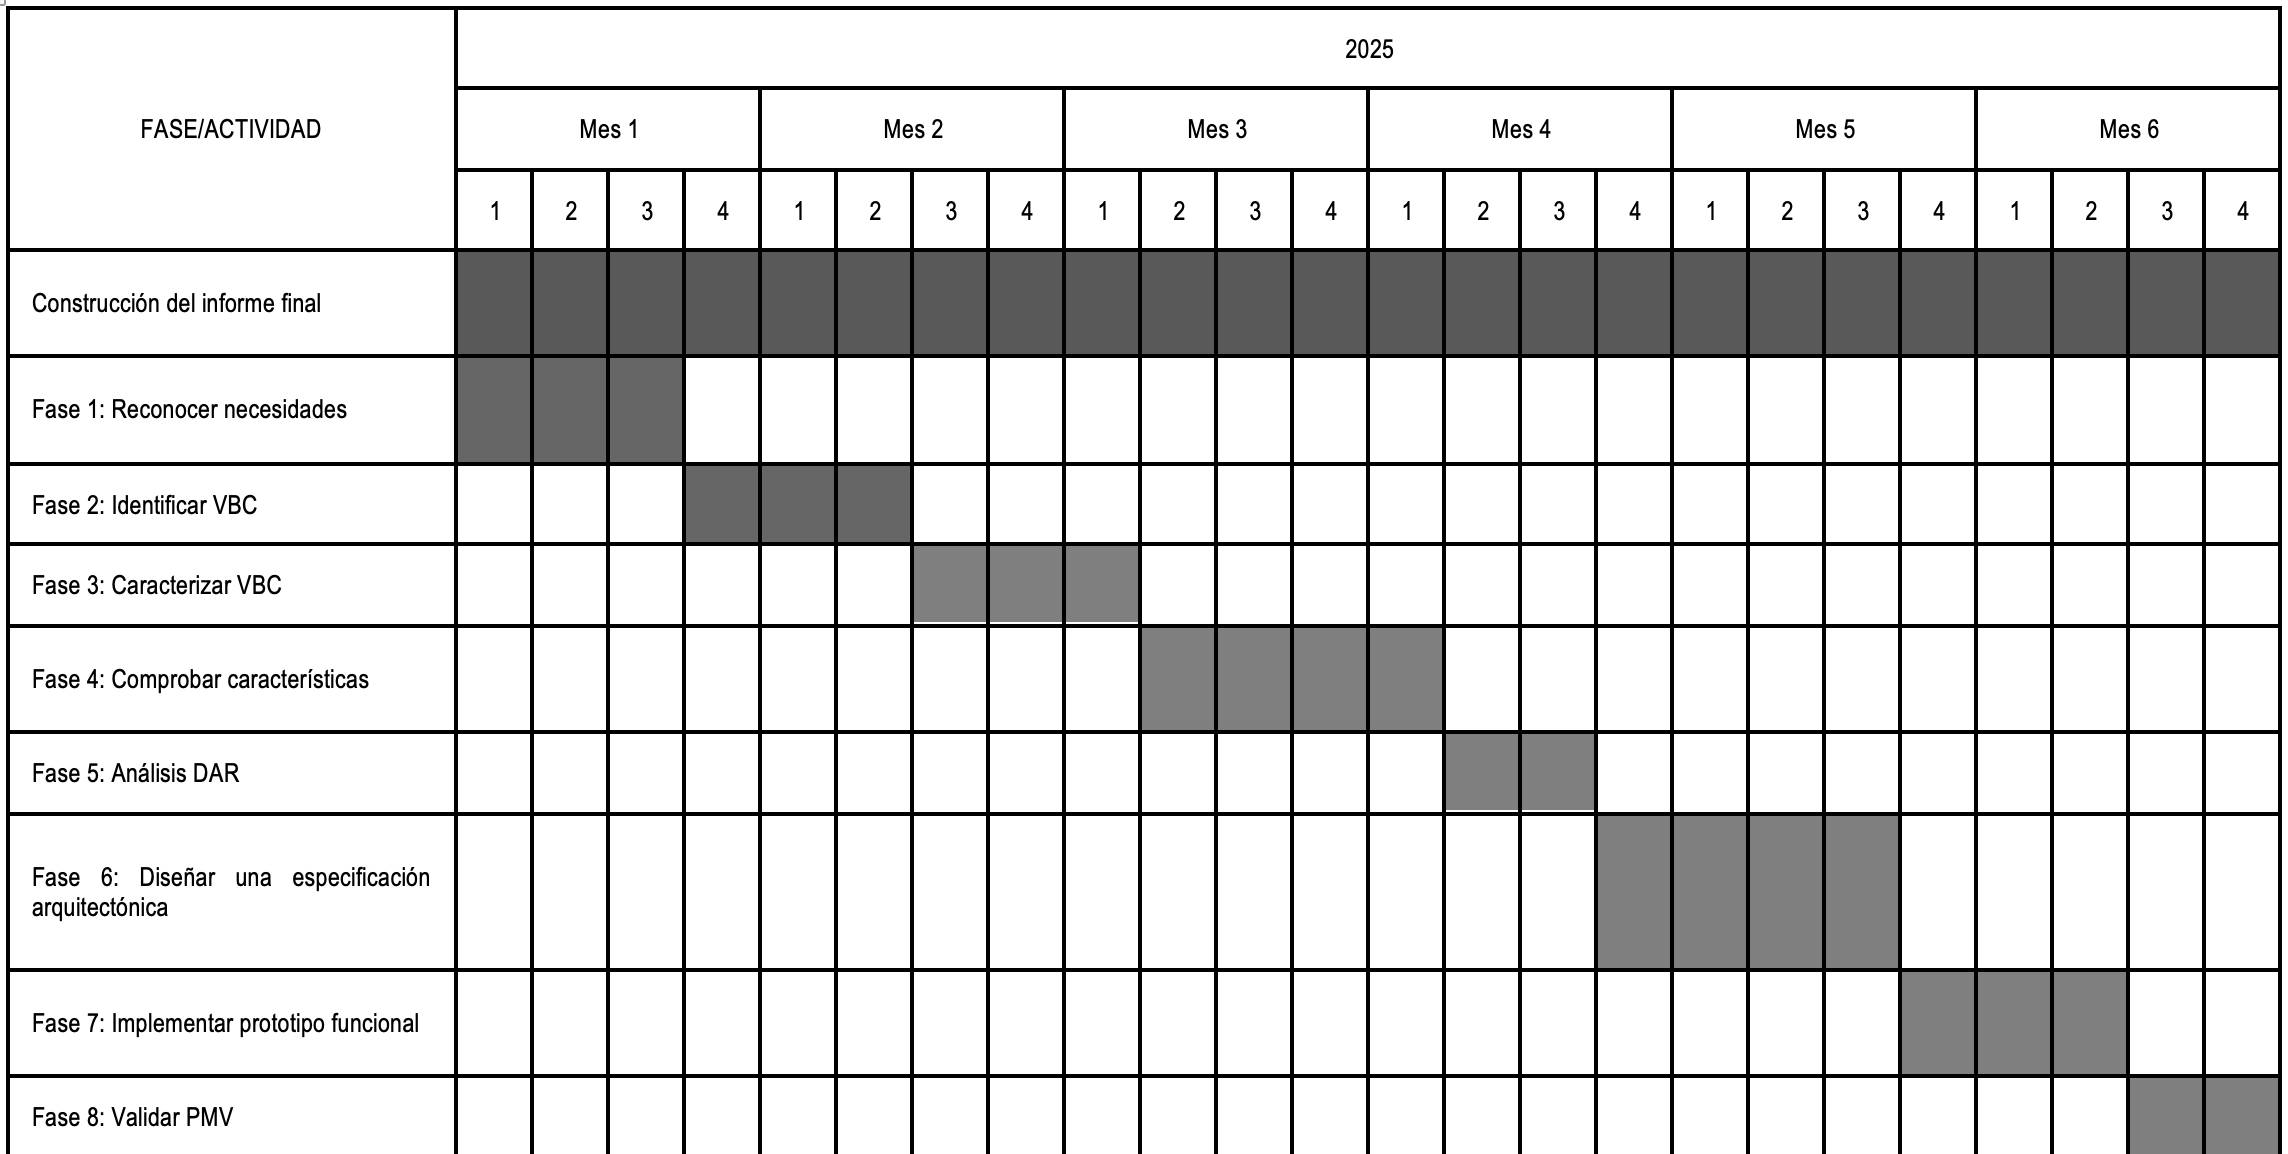
\includegraphics[width=\textwidth]{./tablas-images/cronograma/image.png}
    \caption{Cronograma de actividades del proyecto.}\label{fig:cronograma}
\end{figure}